\documentclass[resume]{subfiles}


\begin{document}
    \section{Courbes et surfaces}
    \subsection{Courbes de Bézier (De Casteljau)}
    \begin{center}
	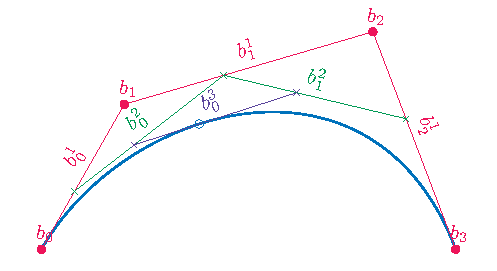
\includegraphics[width=0.6\columnwidth,page=1]{drwg_0.pdf}
	\end{center}
    $$\text{ordre }n \longleftrightarrow n+1\text{ points}$$
	$$\boxed{b_{\text{départ}}^{\text{degré}}}$$
	Exemples :
	\begin{align*}
		\textcolor{RoyalBlue}{b_{0}^{1}(t)}&=(1-t)b_0+tb_1 & b_0\to b_1\\
		\textcolor{OrangeRed}{b_{1}^{1}(t)}&=(1-t)b_1+tb_2 & b_1\to b_2\\
		b_{0}^{2}(t)&=(1-t)\textcolor{RoyalBlue}{b_0^1(t)}+t\textcolor{OrangeRed}{b_1^1(t)} & b_0\to b_2
	\end{align*}
	La courbe de Bézier est comprise dans le polygone de contrôle (points de contrôles reliés).
	\subsection{Polynômes de Bernstein}
	$$\boxed{B_i^n(t)=\begin{pmatrix}
	n\\i
	\end{pmatrix}t^{i}(1-t)^{n-1}\quad i=0,1,...,n\quad t\in[0,1]}$$
	\begin{center}
	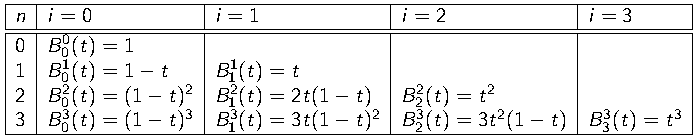
\includegraphics[width=0.8\columnwidth]{img_21.pdf}
	\end{center}
	$$\begin{pmatrix}
	n\\i
	\end{pmatrix}=C_{i}^{n}=\frac{n!}{i!(n-i)!}$$
	La somme des polynômes donne 1
	$$\sum_{i=0}^{n}B_{i}^{n}(t)$$
	\begin{enumerate}
	\item $t=0$ est un zéro de multiplicité $i$
	\item $t=1$ est un zéro de multiplicité $n-i$
	\item $B_{i}^{n}(t)=B_{n-i}^{n}(1-t)$
	\item $B_{i}^{n}(t)=tB_{i-1}^{n-1}(t)+(1-t)B_{i}^{n-1}(t)\qquad i=1,2,...,n-1$
	\end{enumerate}
	Exemples :
	\begin{align*}
	b_0^1(t)&=b_0B_{0}^{1}(t)+b_1B_1^1(t)\\
	b_1^1(t)&=b_1B_0^1(t)+b_2B_1^1(t)\\
	b_0^2(t)&=b_0B_0^2(t)+b_1B_1^2(t)+b_2B_2^2(t)
	\end{align*}
	$$\boxed{x(t)=b_0B_0^3(t)+b_1B_1^3(t)+b_2B_2^3(t)+b_3B_3^3(t)}$$
	\subsection{Bernstein et Bézier}
	$$b_i^r(t)=\sum_{j=0}^{r}b_{i+j}B_j^r(t)$$
	\subsection{Courbes composées}
\begin{enumerate}
\item Deux extrémités égales (points superposés)
\item Points autour de l'extrémité alignés
\end{enumerate}
\begin{figure}[H]
\centering
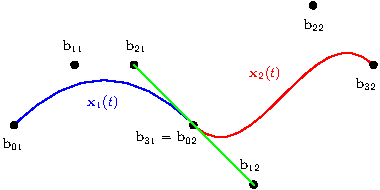
\includegraphics[width=4cm]{img_0.pdf}
\end{figure}



    
\end{document}